\documentclass[12pt, a4paper]{article}
\usepackage[UTF8, zihao=-4]{ctex}
\usepackage[top=2.5cm, bottom=2.5cm, left=2.8cm, right=2.8cm]{geometry}
\usepackage{fontspec}
\setmainfont{Times New Roman}
\usepackage{setspace}
\setstretch{1.5}
\setlength{\parskip}{0pt}
\usepackage{graphicx}
\usepackage{float}
\graphicspath{{实验图片/}}
\usepackage{booktabs}
\usepackage{array}
\usepackage{makecell}
\usepackage{amsmath, amssymb}
\renewcommand{\thefigure}{\arabic{section}-\arabic{figure}}
\renewcommand{\thetable}{\arabic{section}-\arabic{table}}
\counterwithin{figure}{section}
\counterwithin{table}{section}
\usepackage{caption}
\captionsetup{font=small, labelsep=space, justification=centering,
  aboveskip=6pt, belowskip=12pt}
\captionsetup[table]{aboveskip=12pt, belowskip=6pt, position=above}
\usepackage{fancyhdr}
\setlength{\headheight}{15pt}
\pagestyle{fancy}
\fancyhf{}
\fancyhead[C]{\small 刀口阴影法测量光学系统像差综合实验}
\fancyfoot[C]{\small\thepage}
\usepackage[colorlinks=true, linkcolor=black, citecolor=black,
  urlcolor=blue, bookmarks=true, bookmarksnumbered=true]{hyperref}
\usepackage{titlesec}
\titleformat{\section}[block]
  {\centering\heiti\zihao{4}}{\thesection}{1em}{}
\titlespacing*{\section}{0pt}{24pt}{18pt}
\titleformat{\subsection}[hang]
  {\heiti\zihao{-4}}{\thesubsection}{1em}{}
\titlespacing*{\subsection}{0pt}{18pt}{6pt}
\begin{document}
\begin{titlepage}
  \centering
  \vspace*{3cm}
  {\heiti\zihao{2} 实验报告}\\[1cm]
  {\heiti\zihao{3} 刀口阴影法测量光学系统像差综合实验}\\[2cm]
  \begin{tabular}{ll}
    姓\quad 名： & 叶哲昊 \\[0.5cm]
    学\quad 号： & 24012561 \\[0.5cm]
    实验日期：   & 2026年6月5日 \\
  \end{tabular}
  \vfill
\end{titlepage}
\tableofcontents
\newpage
\setcounter{page}{1}
\section{实验目的}
\begin{enumerate}
  \item 巩固光学系统像差理论，加深对球差（Spherical Aberration）和像散（Astigmatism）等几何像差的理解。
  \item 掌握刀口阴影法（Foucault Test）测量光学透镜球差和像散的原理与操作方法。
  \item 通过白屏成像观察并拍摄刀口阴影图样，学会判断刀口与焦点的相对位置关系，定量测量透镜的轴向球差与像散量。
\end{enumerate}
\section{实验原理}
\subsection{刀口阴影法基本原理}
刀口阴影法（Foucault Test）是一种高灵敏度的光学波面检验技术，可灵敏地判别会聚球面波前的完善程度。对于理想成像系统，来自轴上物点的光束经过系统后会聚为理想球面波，所有光线汇聚于球心 $O$ 处。以不透明刀口垂直于光轴方向横向切割成像光束，出现如下三种典型现象：
\begin{itemize}
  \item \textbf{刀口在焦点前}（焦前）：视场中与刀口切入方向\textbf{相同}的一侧出现阴影，对侧保持明亮（"焦前刀影同方向"）。
  \item \textbf{刀口在焦点处}（焦点）：视场整体均匀变暗，无偏暗方向（"焦点阴影一齐暗"）。
  \item \textbf{刀口在焦点后}（焦后）：视场中与刀口切入方向\textbf{相反}的一侧出现阴影（"焦后刀影对面来"）。
\end{itemize}

\subsection{球差测量原理（环带光测试法）}
实际单片正透镜通常存在正球差（欠校正），不同孔径带的光线汇聚于轴上不同位置，边缘光（大孔径）焦点比近轴光焦点更靠近透镜。本实验用环带光阑分别选取直径 10\,mm（近轴区域）和 20\,mm（边缘区域）的光束，分别确定各自的焦点轴向位置 $X_1$（小环带）和 $X_2$（大环带），定义\textbf{轴向球差}为：
\begin{equation}
  \Delta X = X_1 - X_2
  \label{eq:spherical}
\end{equation}
$\Delta X > 0$ 表示近轴光焦点比边缘光焦点距透镜更远，即透镜存在欠校正（正）球差。判断焦点位置的方法：横向移动刀口切入环带光圈，当整个环形光圈同时均匀变暗时，刀口位置即为该环带光对应的轴向焦点，此时读取平移台丝杆读数。

\subsection{球差整体阴影观察}
整体阴影法将刀口置于弥散光斑附近，观察整个光场的阴影分布图样。当系统存在球差时，不同孔径区域光线的聚焦位置不同，阴影图案呈现明暗分区的环状图形，可定性判断球差类型（欠校正或过校正）及其大小。

\subsection{像散测量原理}
当透镜相对于入射光轴有一定倾斜时会产生像散（Astigmatism）。像散的特征是子午焦面（切向焦线，T）与弧矢焦面（矢向焦线，S）在轴向方向相互分离。两焦面分别对应刀口阴影图案呈\textbf{竖直方向}和\textbf{水平方向}的位置，其轴向间距即为\textbf{透镜像散}：
\begin{equation}
  \Delta X_{\mathrm{astig}} = X_2 - X_1
  \label{eq:astig}
\end{equation}
其中 $X_1$ 为子午焦线（刀影竖直）位置读数，$X_2$ 为弧矢焦线（刀影水平）位置读数。像散量随透镜倾斜角的增大而增大。
\section{实验仪器}
本实验所用仪器如下：
\begin{itemize}
  \item LED 光源（波长 690\,nm，红色）
  \item 平行光管（用于产生平行入射光）
  \item 环带光阑（直径 10\,mm 和 20\,mm 两种）
  \item 被测透镜 A（直径 40\,mm，焦距 $f = 200$\,mm，用于球差环带光测试）
  \item 被测透镜 B（直径 40\,mm，焦距 $f = 100$\,mm，用于球差整体阴影观察）
  \item 被测透镜 C（可旋转支架，用于像散测量）
  \item 刀口（精密平移台承载，可横向及纵向移动）
  \item 白屏（因 CCD 接收范围过小，本实验统一以白屏替代 CMOS 相机，结合相机拍照记录）
  \item 精密导轨及平移台（丝杆读数，分度值约 0.01\,mm）
\end{itemize}
\section{实验步骤}
\subsection{球差测量（环带光测试法）}
\begin{enumerate}
  \item 按如下光路搭建系统：LED 光源 $\to$ 平行光管 $\to$ 10\,mm 环带光阑 $\to$ 被测透镜 A（$f=200$\,mm）$\to$ 刀口 $\to$ 白屏，调节各元件共轴。
  \item 在白屏上观察到清晰的圆形环带光圈后，精细移动平移台改变刀口的纵向位置，分别在焦前、焦点和焦后观察阴影图样变化，拍照记录。
  \item 调节刀口至使小环带光圈\textbf{同时均匀变暗}的位置，读取平移台丝杆示数 $X_1$，记入数据表格。
  \item 换用 20\,mm 环带光阑，重新调节刀口，找到大环带光圈同时均匀变暗的位置，记录丝杆示数 $X_2$。
  \item 重复测量 3 次（每次重新从焦前或焦后趋近焦点），计算每次轴向球差 $\Delta X = X_1 - X_2$，取平均值。
\end{enumerate}

\subsection{球差整体阴影观察}
\begin{enumerate}
  \item 去掉环带光阑，换用被测透镜 B（$f=100$\,mm），光路：LED 光源 $\to$ 平行光管 $\to$ 透镜 B $\to$ 刀口 $\to$ 白屏。
  \item 调节刀口至透镜后方焦点弥散斑附近，横向切割成像光束，观察白屏上出现的整体阴影图样。
  \item 缓慢前后移动平移台，观察阴影图案随刀口位置变化的规律，拍照记录有代表性的图样。
\end{enumerate}

\subsection{像散测量}
\begin{enumerate}
  \item 恢复 10\,mm 环带光阑，换用带旋转支架的被测透镜 C，光路：LED 光源 $\to$ 平行光管 $\to$ 10\,mm 环带光阑 $\to$ 旋转透镜 C $\to$ 刀口 $\to$ 白屏。
  \item 将透镜 C 相对光轴旋转 $20°$，前后移动刀口，当白屏上出现\textbf{竖直方向}（子午焦线）阴影时，记录平移台读数 $X_1$；继续移动刀口至出现\textbf{水平方向}（弧矢焦线）阴影，记录读数 $X_2$。
  \item 在旋转角度 $20°$、$30°$、$40°$ 下分别重复上述步骤，记录各角度下的 $X_1$、$X_2$ 和像散量 $\Delta X = X_2 - X_1$。
\end{enumerate}
\section{实验数据与处理}
\subsection{轴向球差测量数据}
实验中选用 10\,mm（小环带，对应近轴光区）和 20\,mm（大环带，对应边缘光区）两种环带光阑，分别定位各自焦点的轴向位置，三次测量结果如表~\ref{tab:spherical}所示。

\begin{table}[H]
  \centering
  \caption{红色光源轴向球差（环带光测试法，$\lambda = 690$\,nm）}
  \label{tab:spherical}
  \begin{tabular}{cccc}
    \toprule
    次数 & \makecell{$X_1$/mm\\（小环带，10\,mm）} & \makecell{$X_2$/mm\\（大环带，20\,mm）} & \makecell{轴向球差\\$\Delta X = X_1 - X_2$/mm} \\
    \midrule
    1 & 11.520 & 8.018 & 3.502 \\
    2 & 10.522 & 7.834 & 2.688 \\
    3 & 10.515 & 7.935 & 2.580 \\
    \midrule
    平均值 & — & — & 2.923 \\
    \bottomrule
  \end{tabular}
\end{table}

轴向球差均值为：
\begin{equation}
  \overline{\Delta X} = \frac{3.502 + 2.688 + 2.580}{3} \approx 2.923\,\text{mm}
  \label{eq:spherical_avg}
\end{equation}

\subsection{像散测量数据}
将透镜分别旋转 $20°$、$30°$、$40°$，分别寻找子午焦线（刀影竖直）和弧矢焦线（刀影水平）的轴向位置，数据如表~\ref{tab:astig}所示。

\begin{table}[H]
  \centering
  \caption{透镜像散数据记录}
  \label{tab:astig}
  \begin{tabular}{cccc}
    \toprule
    旋转角度 & \makecell{$X_1$/mm\\（子午焦线，刀影竖直）} & \makecell{$X_2$/mm\\（弧矢焦线，刀影水平）} & \makecell{像散\\$\Delta X = X_2 - X_1$/mm} \\
    \midrule
    $20°$ & 761.9 & 811.5 & 49.6 \\
    $30°$ & 731.8 & 797.5 & 65.7 \\
    $40°$ & 698.1 & 775.0 & 76.9 \\
    \midrule
    平均值 & — & — & 64.1 \\
    \bottomrule
  \end{tabular}
\end{table}

像散均值为：
\begin{equation}
  \overline{\Delta X}_{\mathrm{astig}} = \frac{49.6 + 65.7 + 76.9}{3} \approx 64.1\,\text{mm}
  \label{eq:astig_avg}
\end{equation}

由表~\ref{tab:astig}可以看出，随透镜旋转角度增大，子午焦线与弧矢焦线之间的轴向距离显著增大，即像散量随倾斜角增大而增大，与理论预测一致。
\section{实验结果与分析}
\subsection{球差观察结果（环带光测试法）}
图~\ref{fig:sphere_focus}展示了小环带（10\,mm）和大环带（20\,mm）在刀口切入焦点时白屏上的阴影图样，两种情形均呈现环带光圈同时均匀变暗的特征，确认了各自焦点位置的准确性。两种环带光阑对应焦点位置之差即为轴向球差，验证了正透镜欠校正球差的存在。

\begin{figure}[H]
  \centering
  \begin{minipage}{0.48\textwidth}
    \centering
    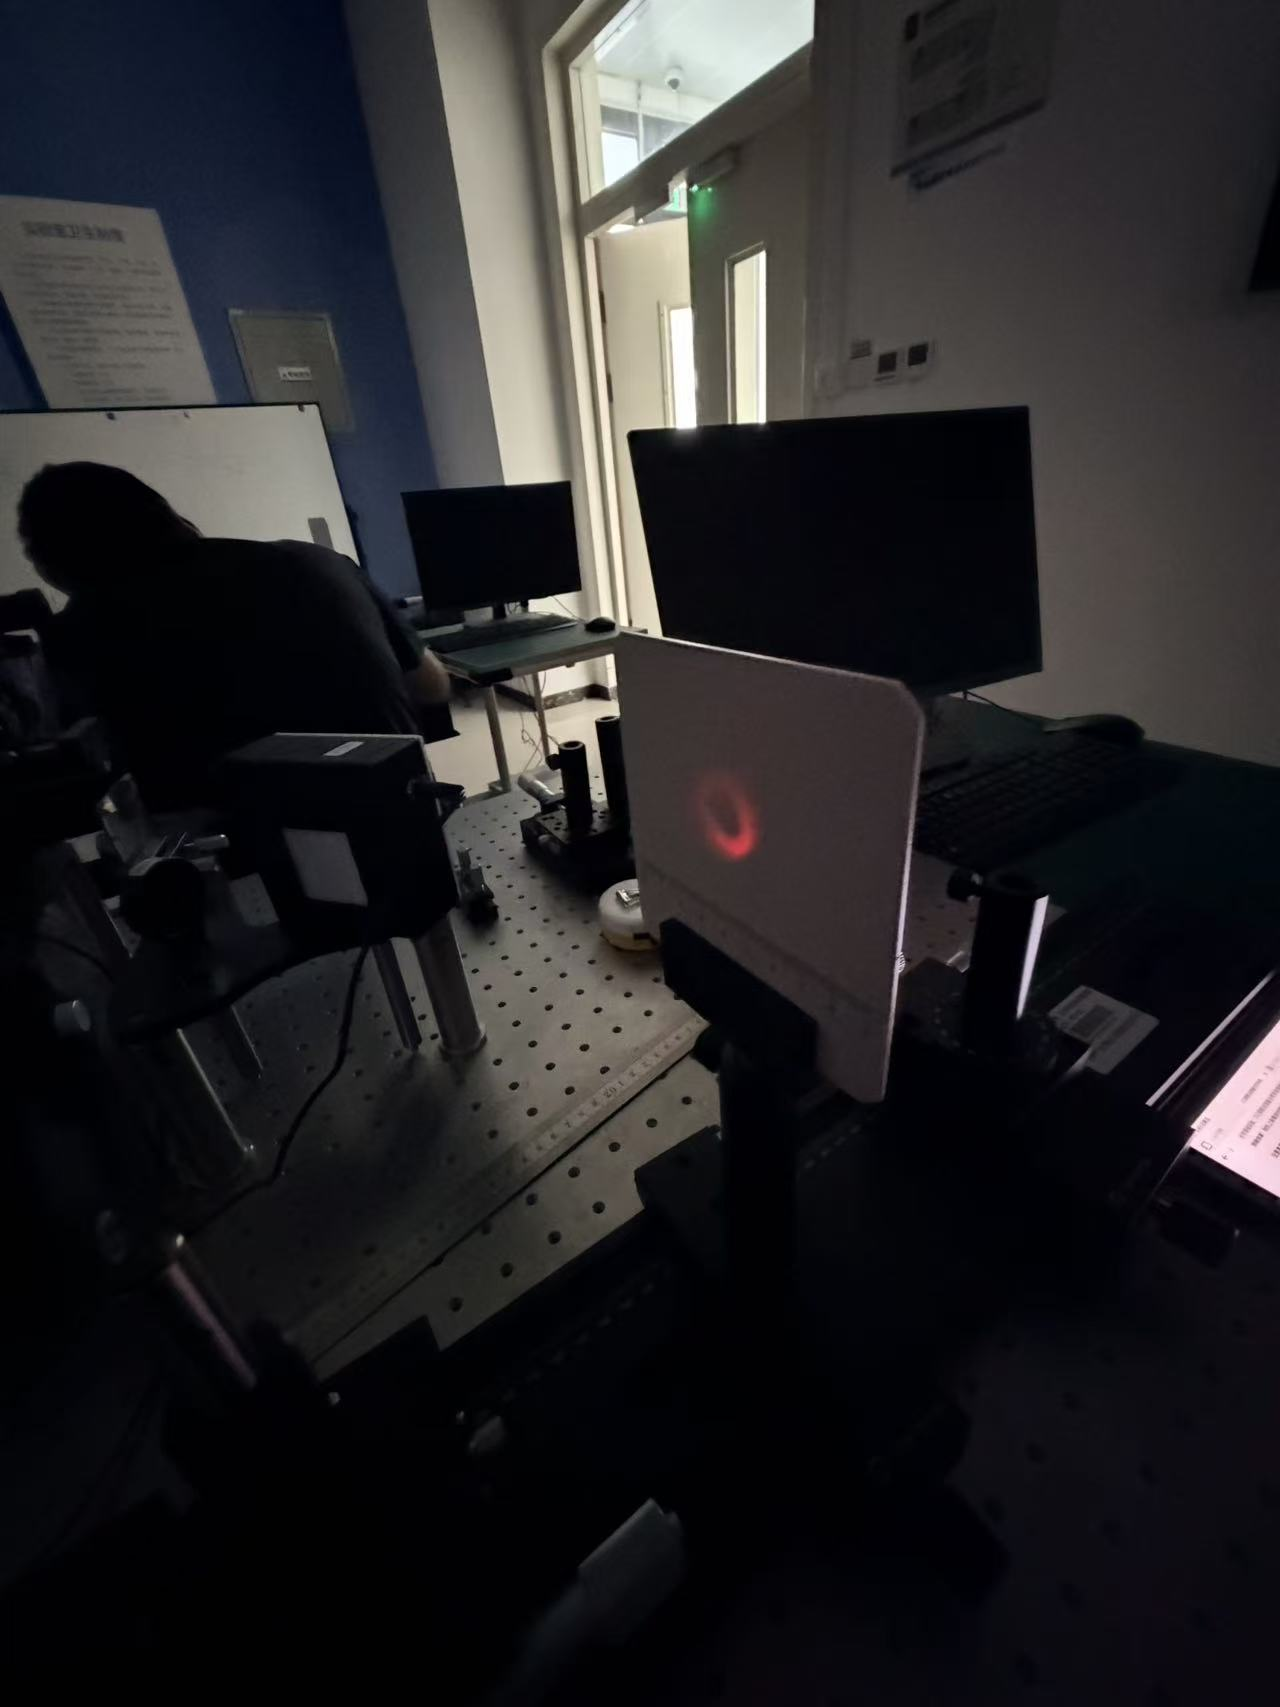
\includegraphics[width=\textwidth]{小的环带光阑，在焦点上，切入，图像同时变暗.jpg}
    \caption*{(a) 小环带（10\,mm），刀口位于焦点处，光圈同时变暗}
  \end{minipage}
  \hfill
  \begin{minipage}{0.48\textwidth}
    \centering
    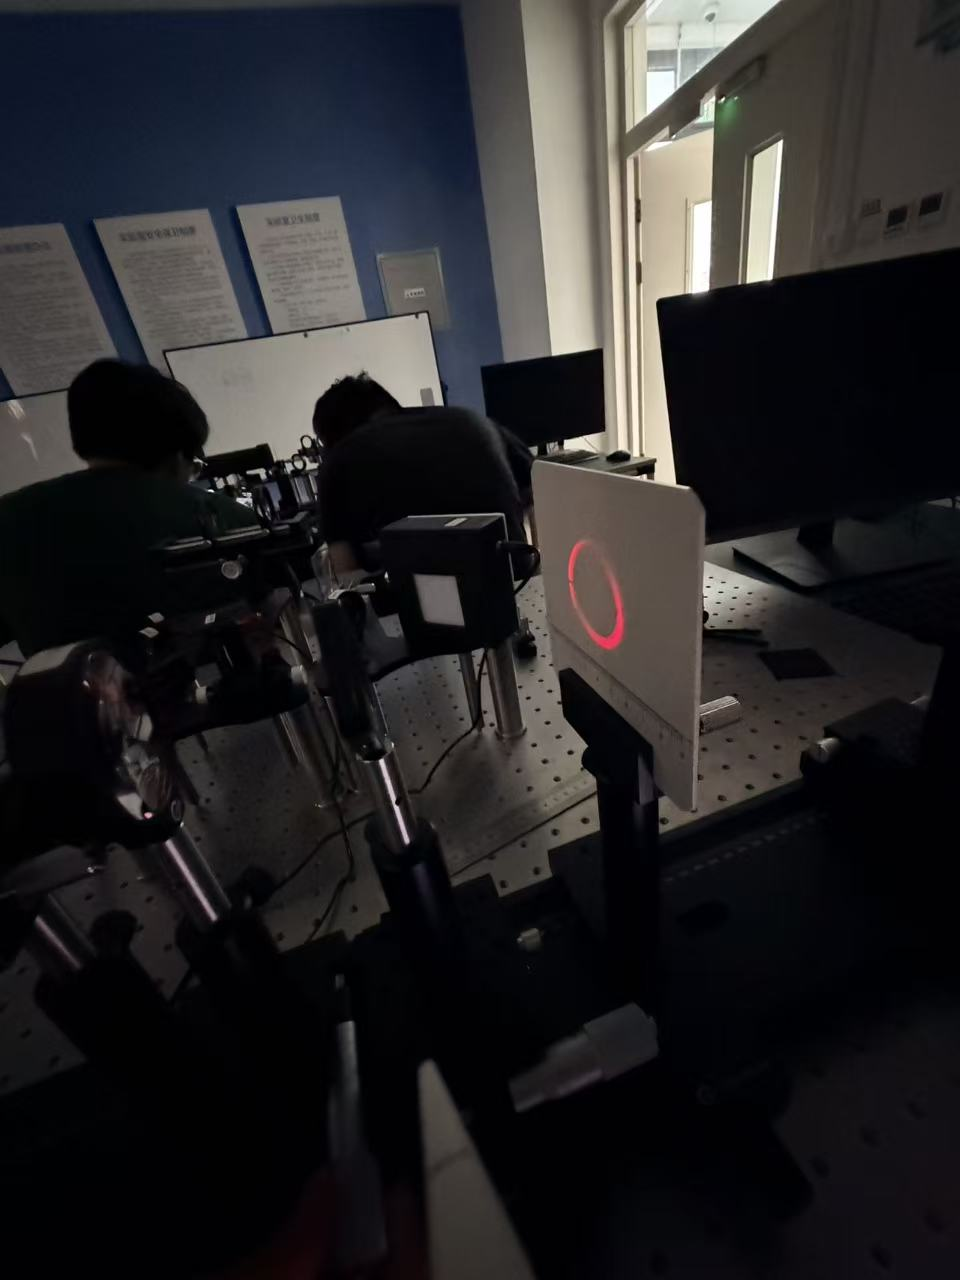
\includegraphics[width=\textwidth]{大的环带光阑，焦点切入，同时变暗.jpg}
    \caption*{(b) 大环带（20\,mm），刀口位于焦点处，光圈同时变暗}
  \end{minipage}
  \caption{两种环带光阑在焦点处的刀口阴影图样（白屏观察）}
  \label{fig:sphere_focus}
\end{figure}

\begin{figure}[H]
  \centering
  \begin{minipage}{0.48\textwidth}
    \centering
    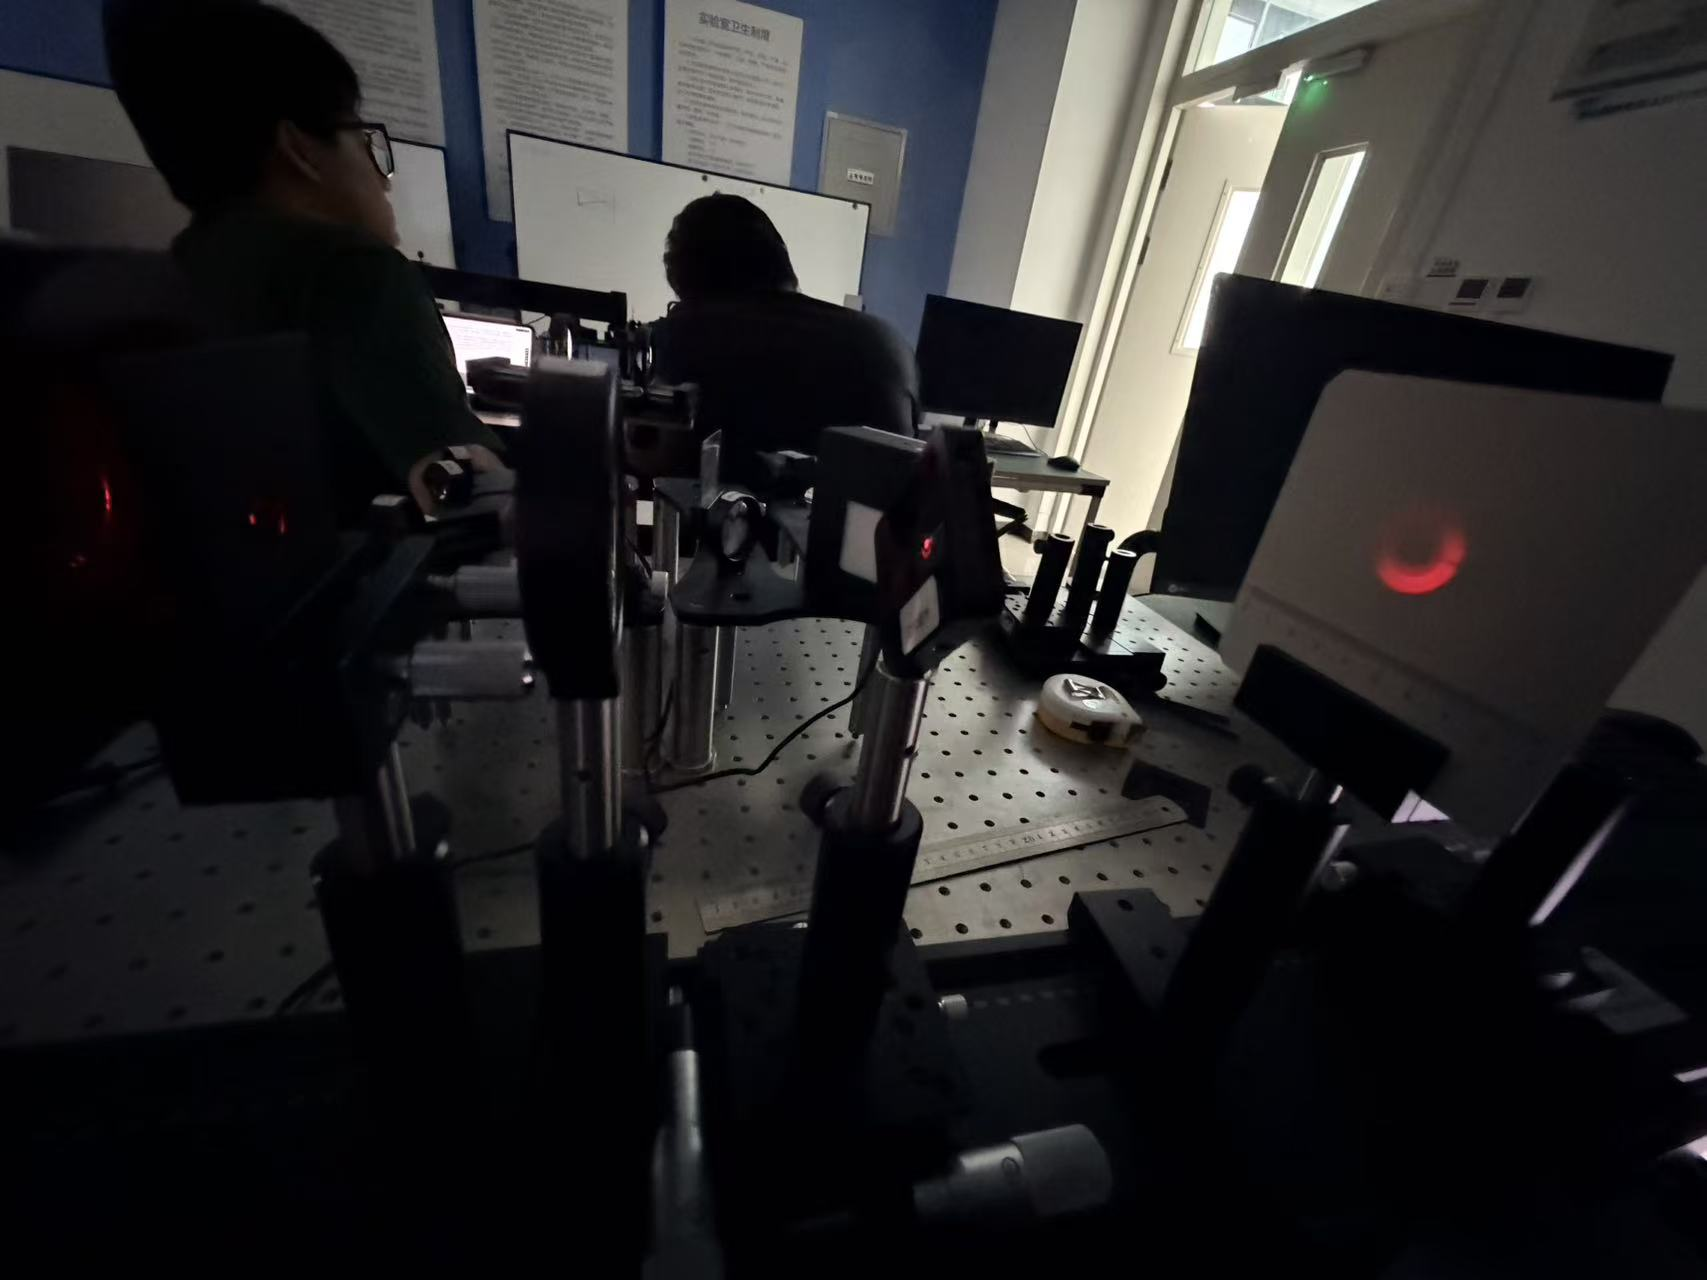
\includegraphics[width=\textwidth]{小的环带光阑，切入，反侧变暗.jpg}
    \caption*{(a) 刀口在焦前，对侧（反侧）变暗}
  \end{minipage}
  \hfill
  \begin{minipage}{0.48\textwidth}
    \centering
    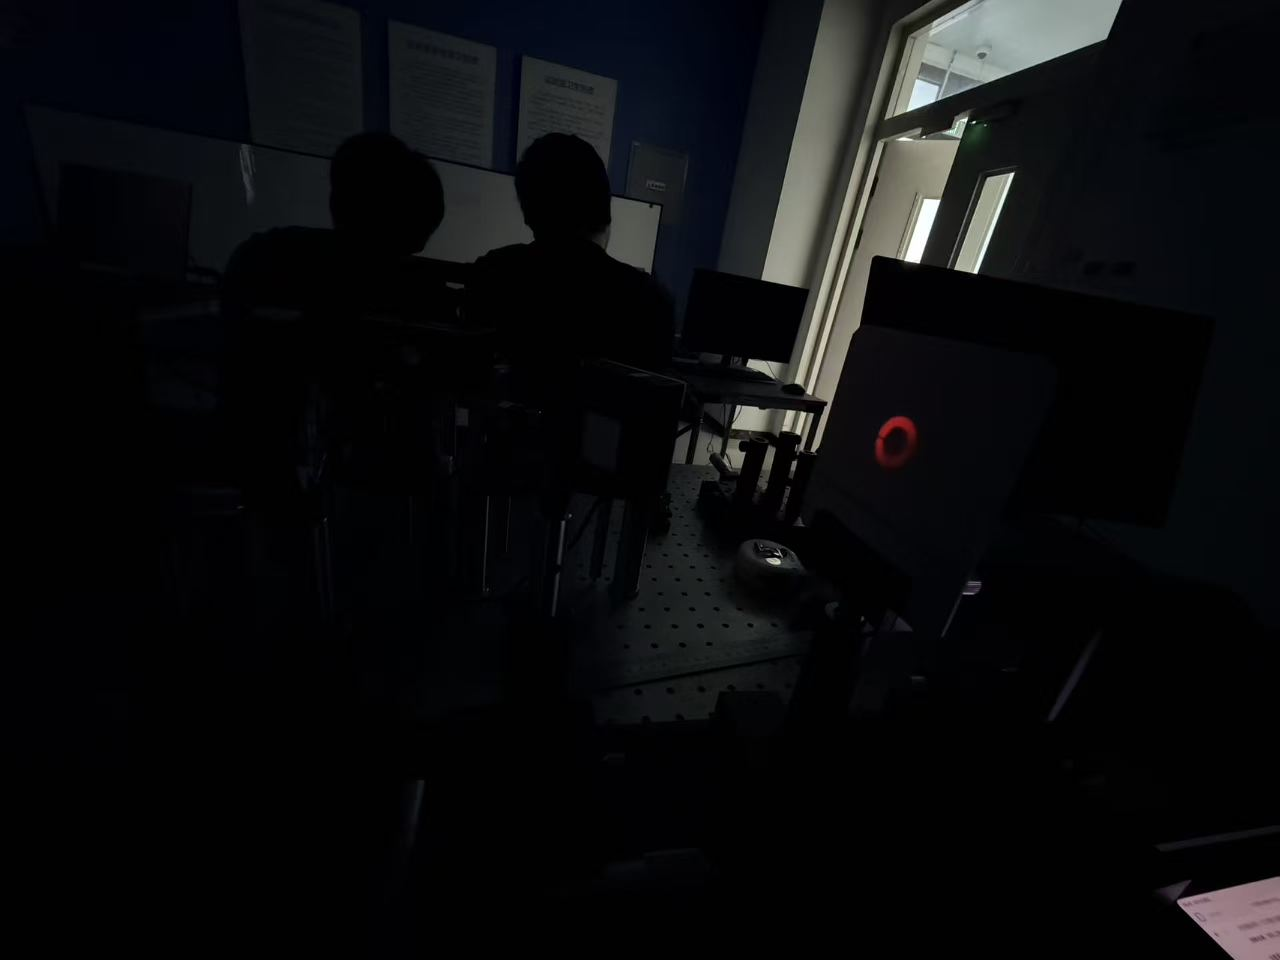
\includegraphics[width=\textwidth]{小的环带光阑，在焦后，切入，正侧变暗.jpg}
    \caption*{(b) 刀口在焦后，同侧（正侧）变暗}
  \end{minipage}
  \caption{刀口在焦前和焦后时的阴影图样对比（小环带，白屏观察）}
  \label{fig:sphere_pre_post}
\end{figure}

\subsection{球差整体阴影观察结果}
图~\ref{fig:sphere_overall}为整体阴影法实验现场照片。可在白屏（图中右侧屏幕）上观察到因球差引起的环状阴影图案，直观展示了正透镜弥散光场中不同孔径区域光线聚焦位置不一致的现象。

\begin{figure}[H]
  \centering
  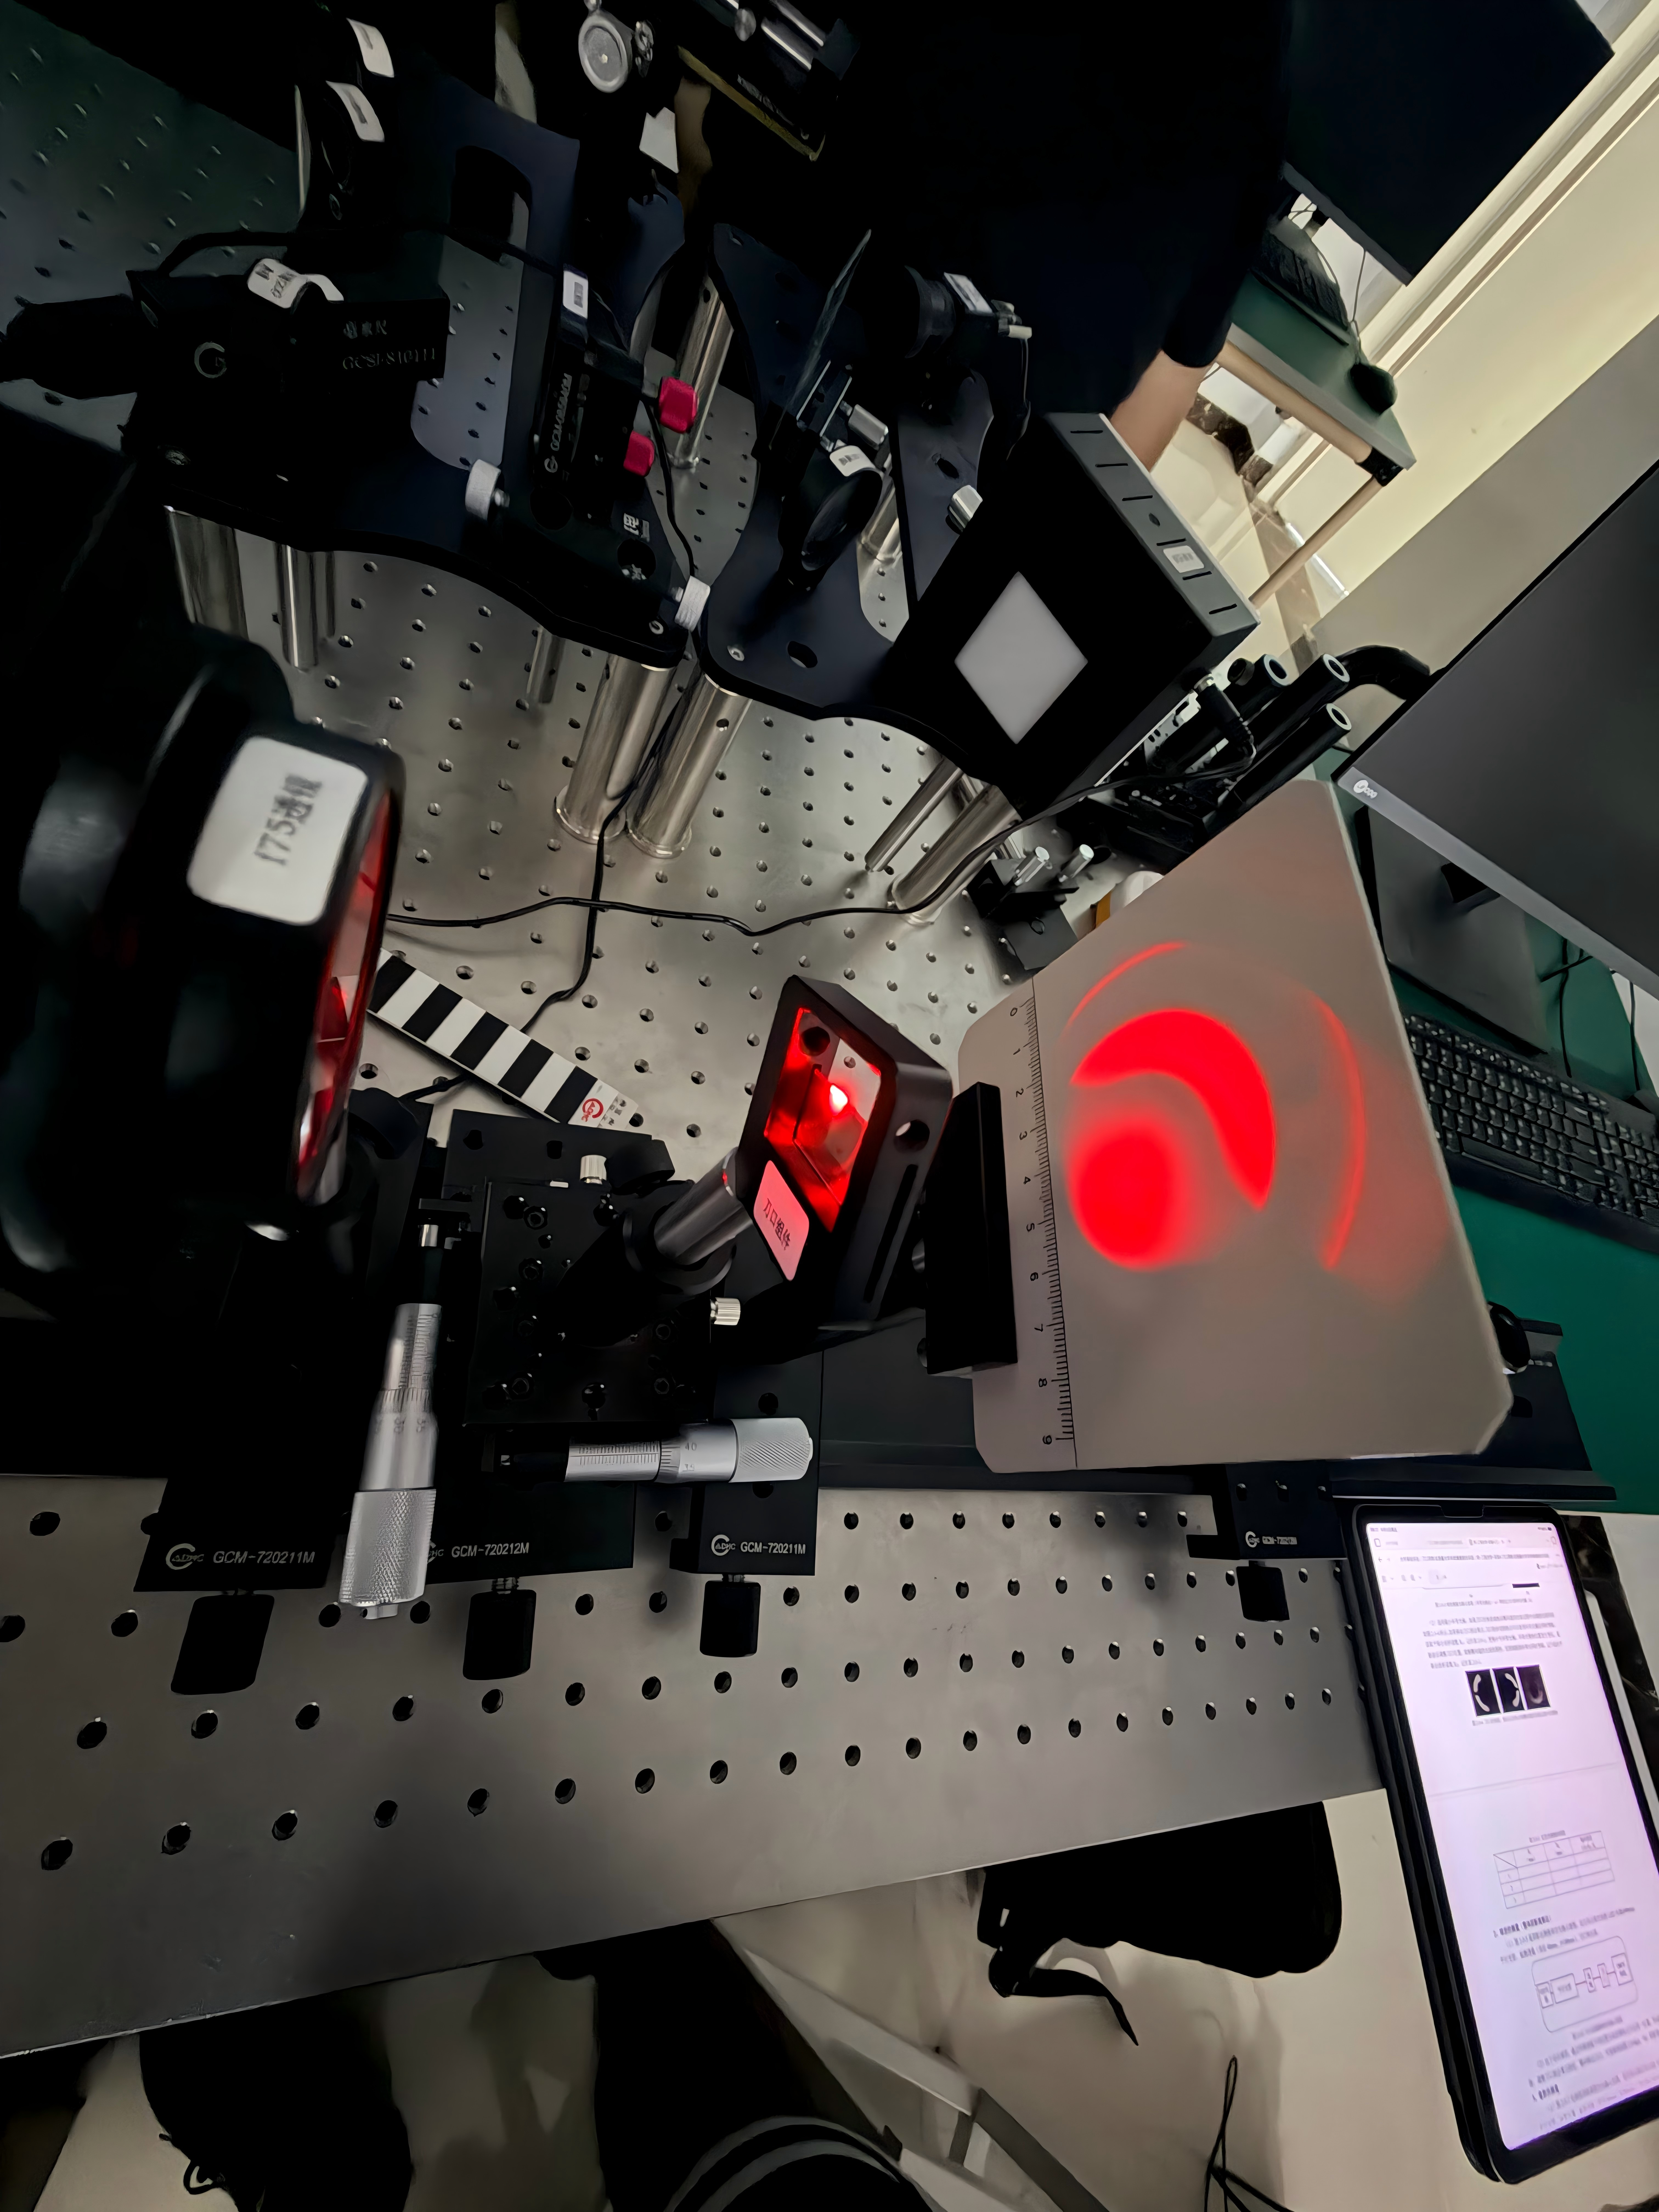
\includegraphics[width=0.65\textwidth]{整体法观察像散的照片.jpg}
  \caption{整体阴影法实验现场照片（白屏上可见环状阴影图案）}
  \label{fig:sphere_overall}
\end{figure}

\subsection{像散观察结果}
图~\ref{fig:astig_20}至图~\ref{fig:astig_40}分别展示了透镜旋转 $20°$、$30°$、$40°$ 时，刀口在子午焦线与弧矢焦线处的阴影图样。竖直阴影对应子午焦线（$X_1$），水平阴影对应弧矢焦线（$X_2$）。

\begin{figure}[H]
  \centering
  \begin{minipage}{0.48\textwidth}
    \centering
    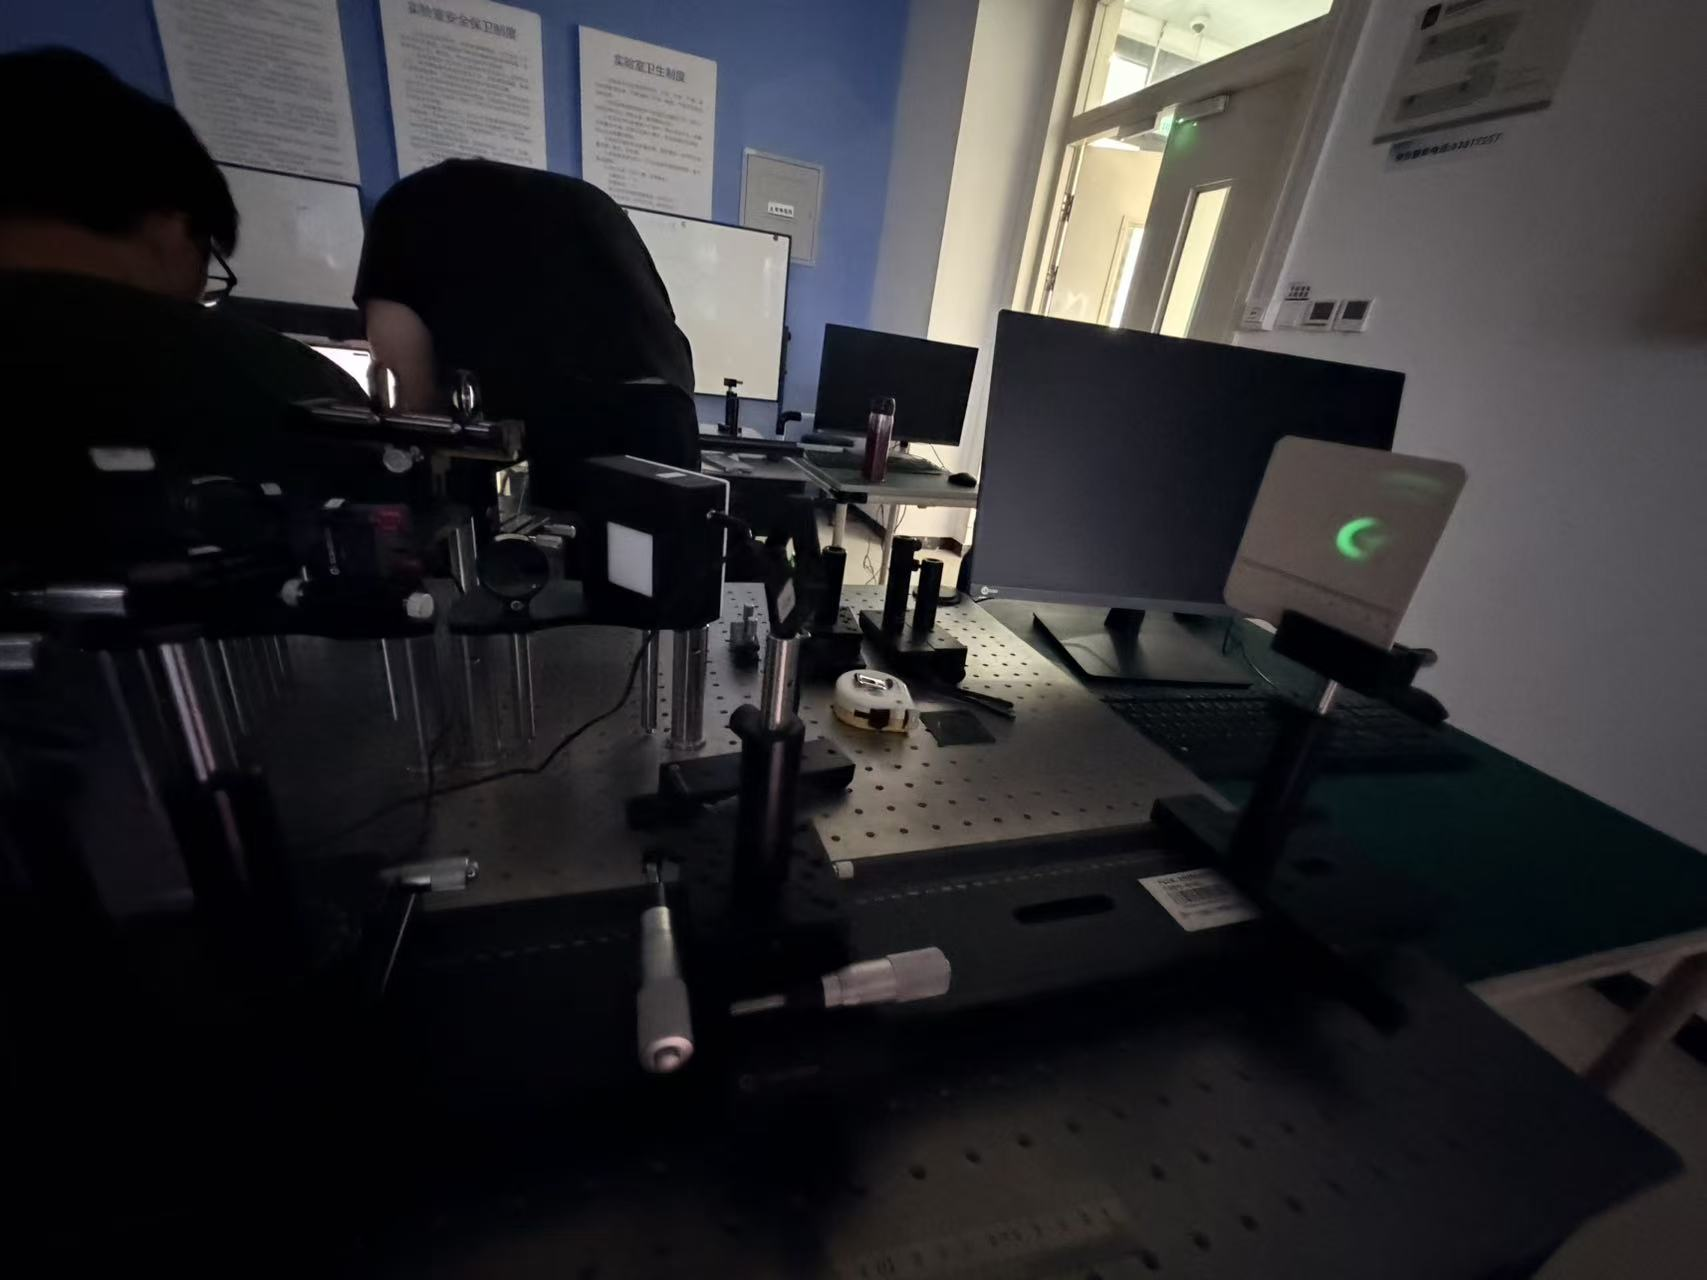
\includegraphics[width=\textwidth]{像散，20度，竖着切.jpg}
    \caption*{(a) 旋转 $20°$，子午焦线，$X_1=761.9$\,mm}
  \end{minipage}
  \hfill
  \begin{minipage}{0.48\textwidth}
    \centering
    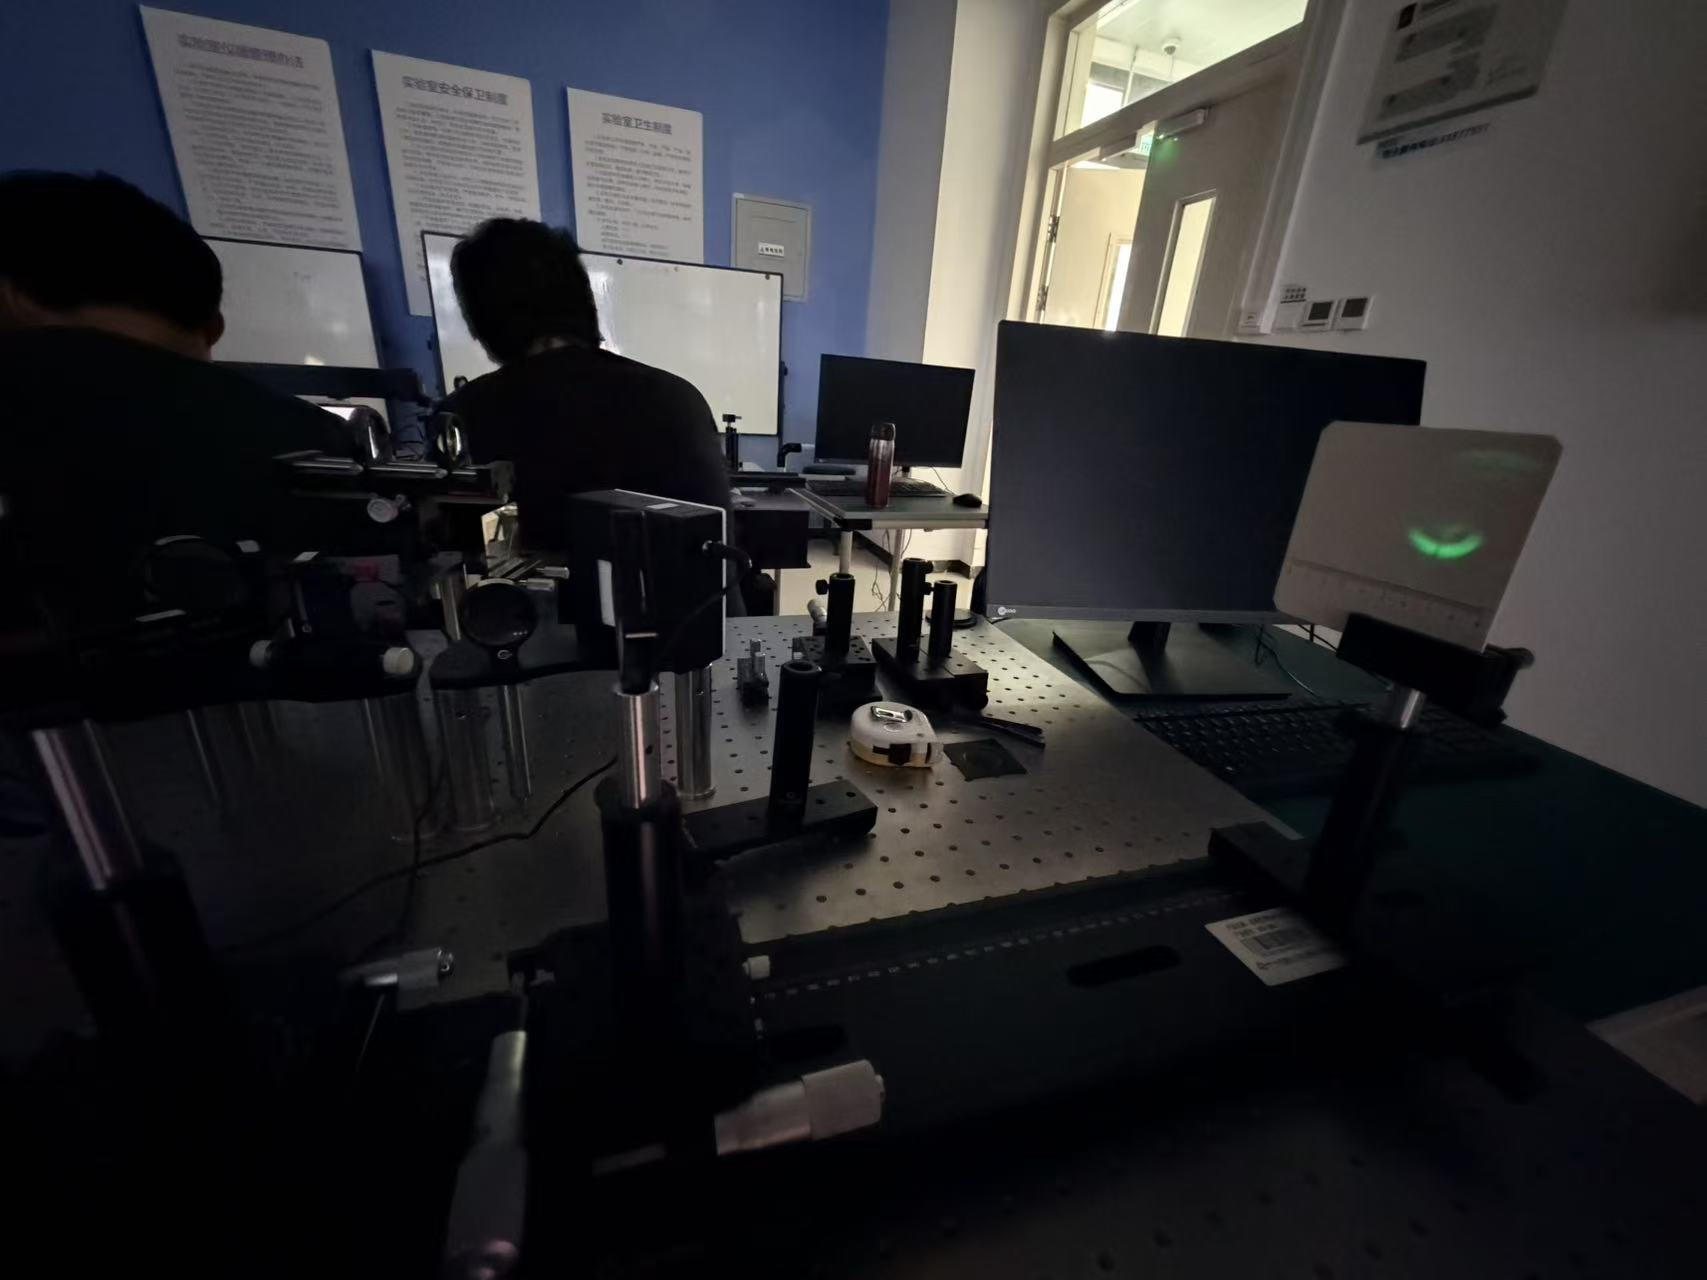
\includegraphics[width=\textwidth]{像散，20度，横着切.jpg}
    \caption*{(b) 旋转 $20°$，弧矢焦线，$X_2=811.5$\,mm}
  \end{minipage}
  \caption{旋转 $20°$ 时的像散刀口阴影图样，$\Delta X=49.6$\,mm（白屏观察）}
  \label{fig:astig_20}
\end{figure}

\begin{figure}[H]
  \centering
  \begin{minipage}{0.48\textwidth}
    \centering
    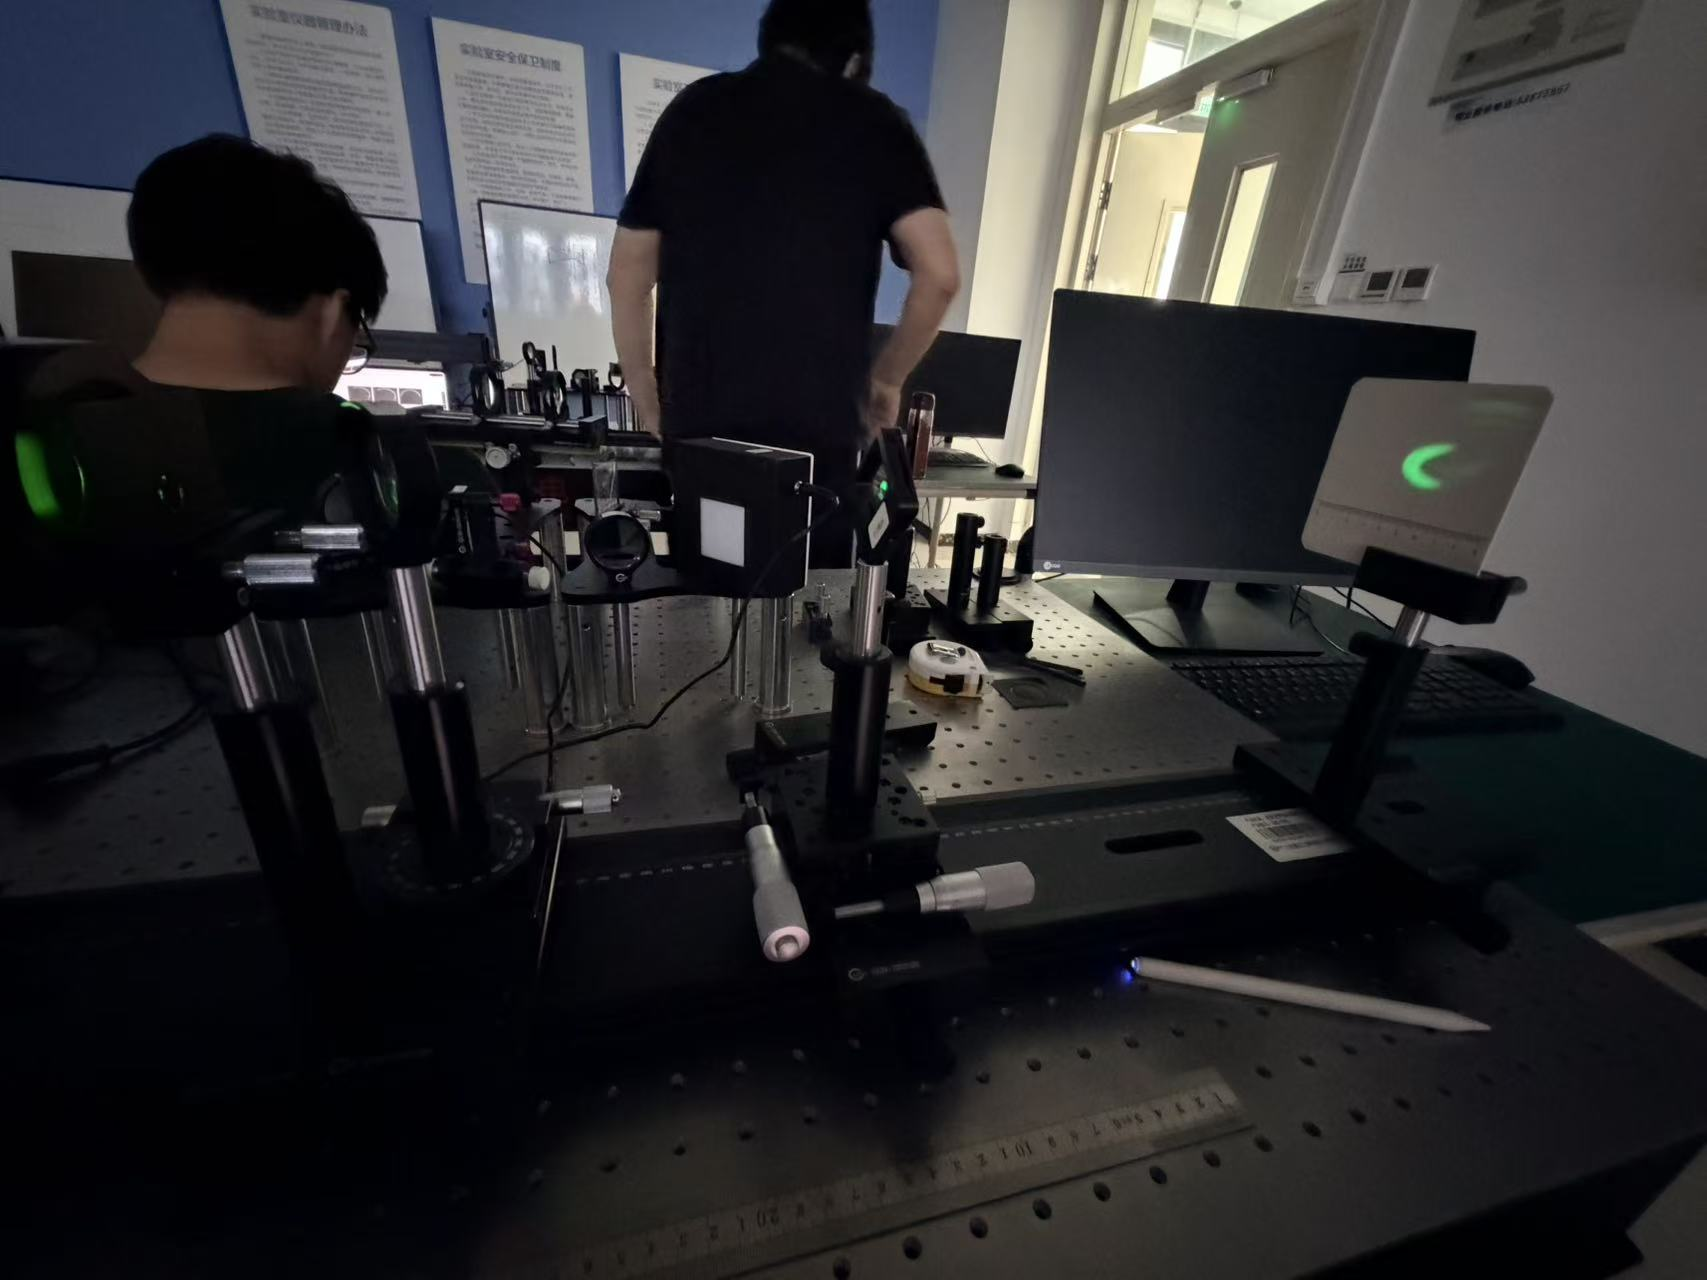
\includegraphics[width=\textwidth]{像散，30度，竖着切.jpg}
    \caption*{(a) 旋转 $30°$，子午焦线，$X_1=731.8$\,mm}
  \end{minipage}
  \hfill
  \begin{minipage}{0.48\textwidth}
    \centering
    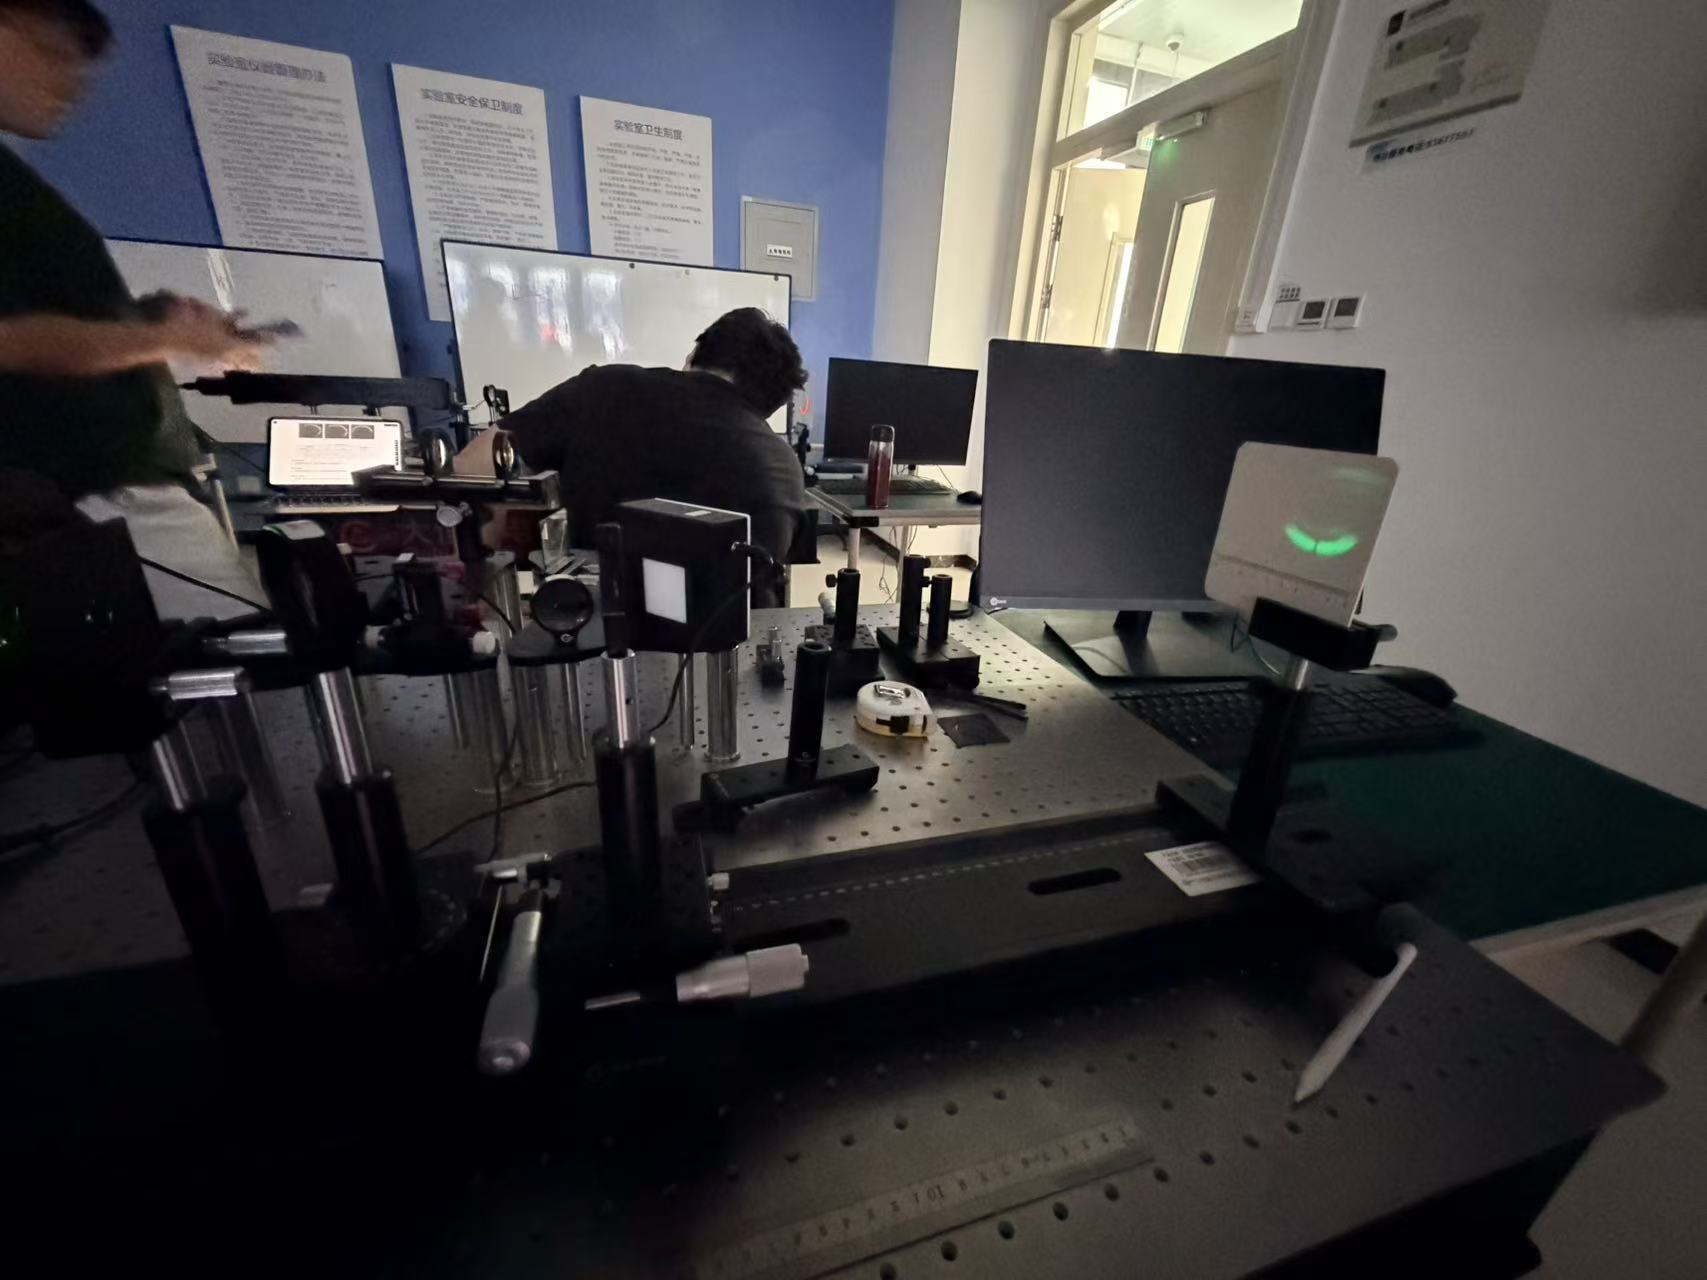
\includegraphics[width=\textwidth]{像散，30度，水平切.jpg}
    \caption*{(b) 旋转 $30°$，弧矢焦线，$X_2=797.5$\,mm}
  \end{minipage}
  \caption{旋转 $30°$ 时的像散刀口阴影图样，$\Delta X=65.7$\,mm（白屏观察）}
  \label{fig:astig_30}
\end{figure}

\begin{figure}[H]
  \centering
  \begin{minipage}{0.48\textwidth}
    \centering
    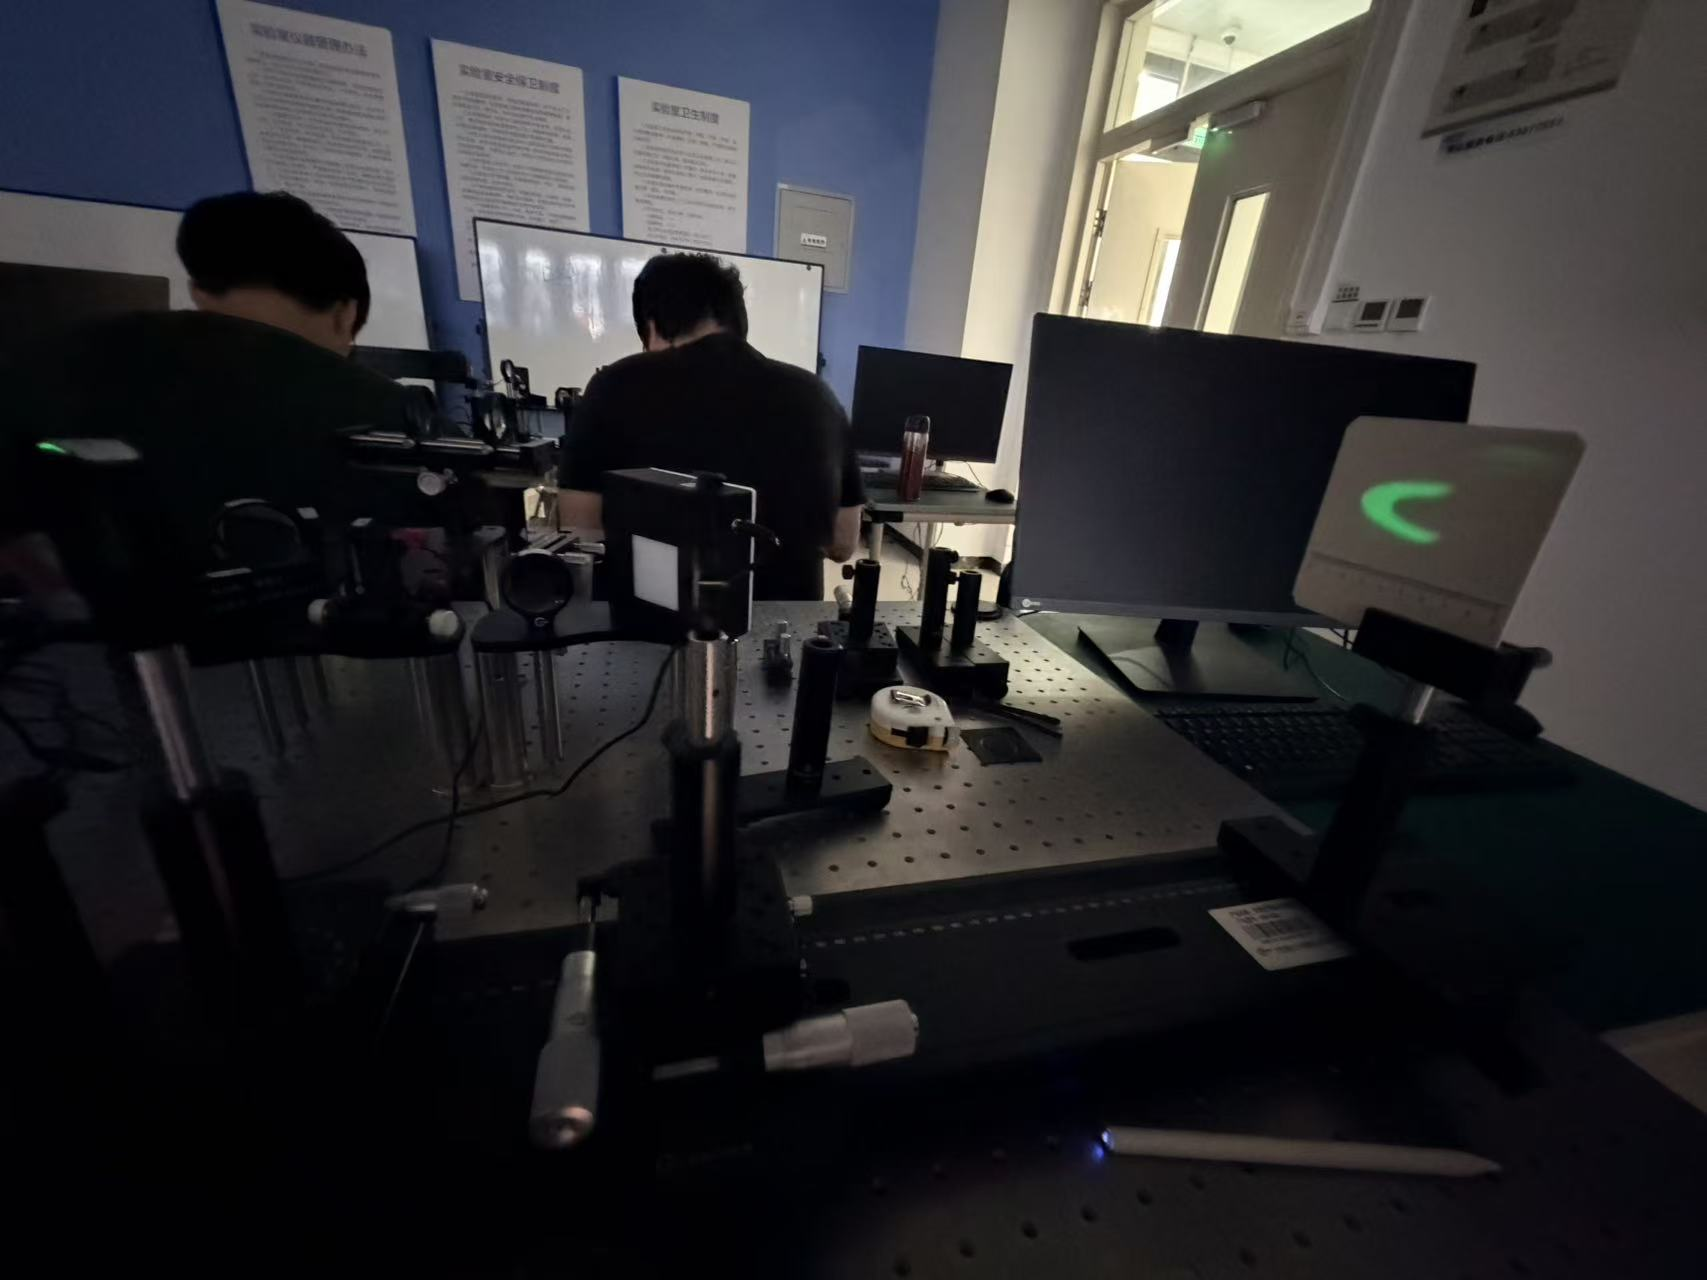
\includegraphics[width=\textwidth]{像散，40度，竖着切.jpg}
    \caption*{(a) 旋转 $40°$，子午焦线，$X_1=698.1$\,mm}
  \end{minipage}
  \hfill
  \begin{minipage}{0.48\textwidth}
    \centering
    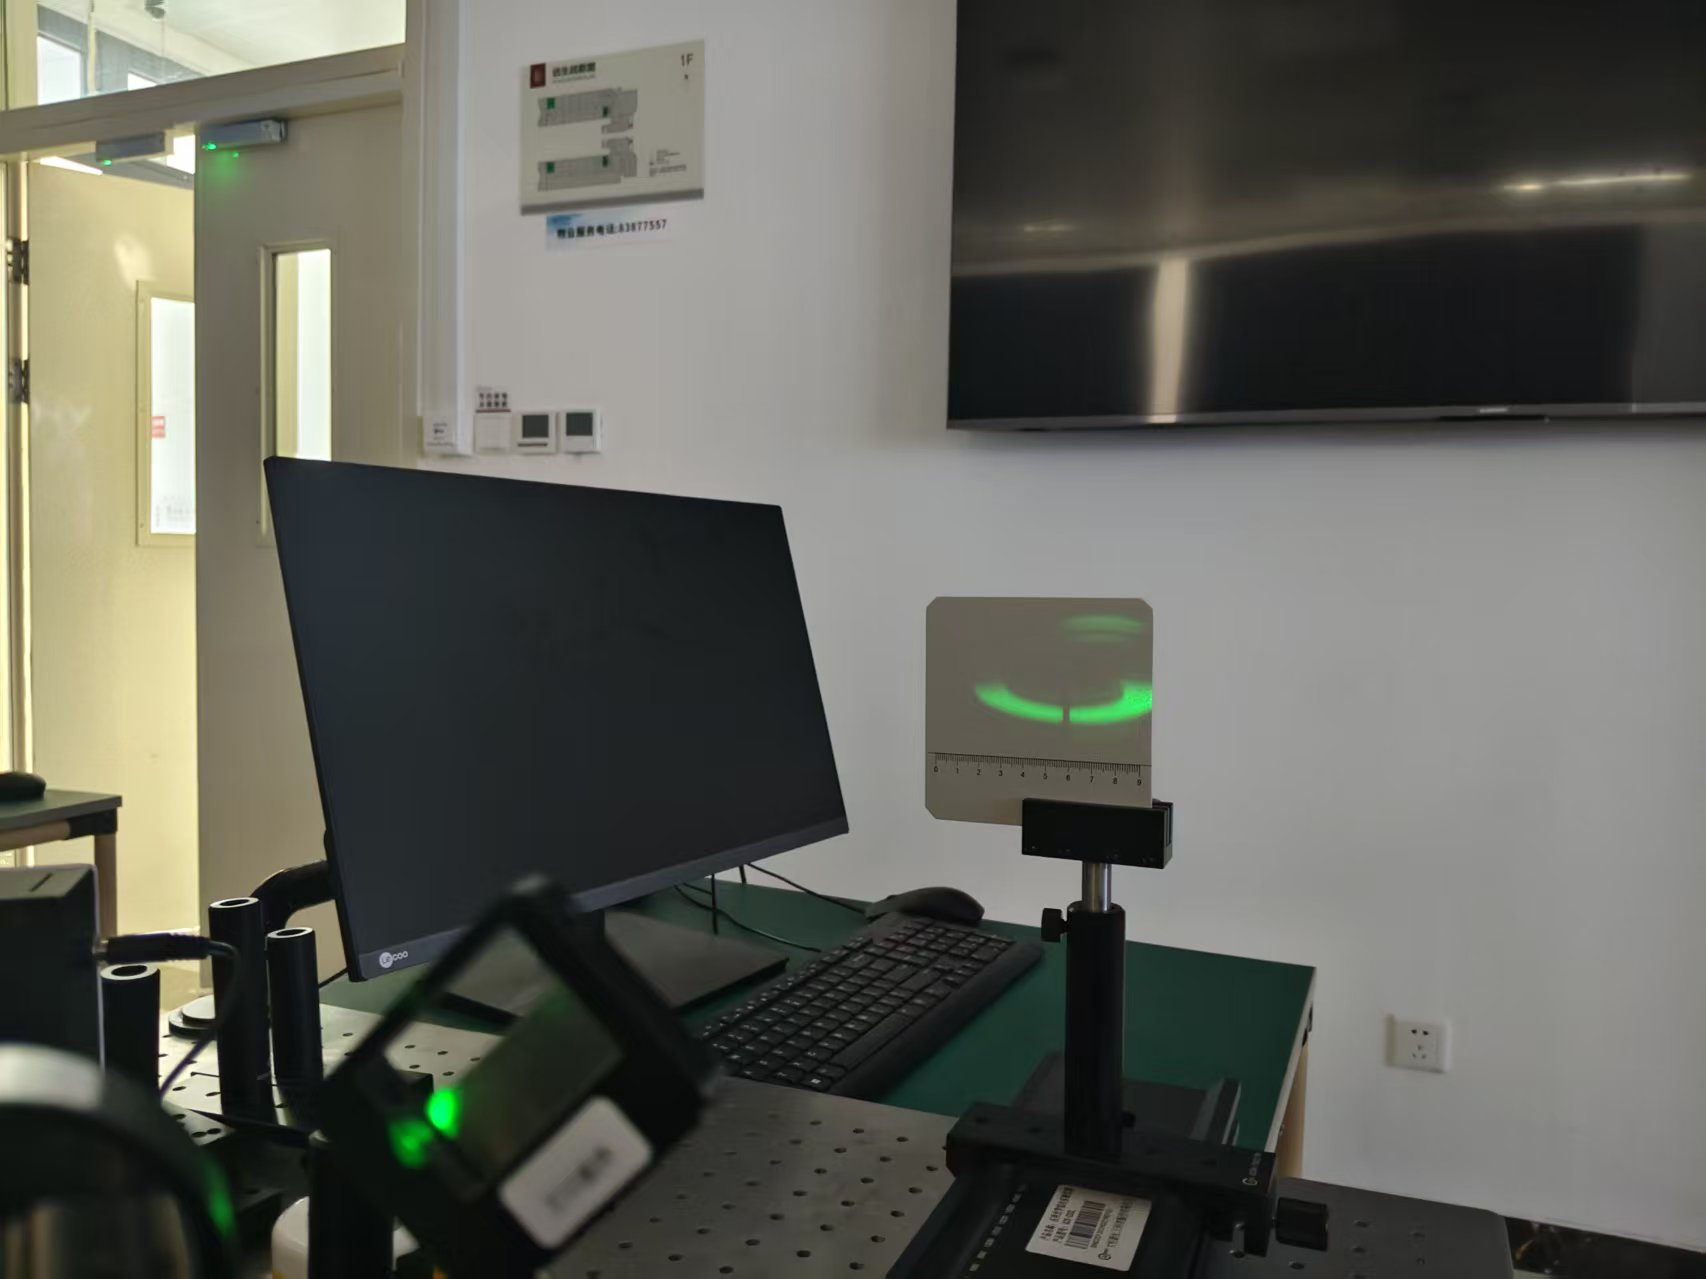
\includegraphics[width=\textwidth]{像散，40度，横着切.jpg}
    \caption*{(b) 旋转 $40°$，弧矢焦线，$X_2=775.0$\,mm}
  \end{minipage}
  \caption{旋转 $40°$ 时的像散刀口阴影图样，$\Delta X=76.9$\,mm（白屏观察）}
  \label{fig:astig_40}
\end{figure}
\section{误差分析}
本实验的测量误差主要来源于以下几个方面：
\begin{enumerate}
  \item \textbf{人眼判断误差}：确定刀口位于焦点的标准是环带光圈“同时均匀变暗”，这一判断完全依赖人眼对亮度均匀性的感知，个体差异和疲劳度均会带来偏差。
  \item \textbf{平移台机械误差}：丝杆存在回程差，若多次测量时趋近方向不一致，读数偏差可达数分之一毫米。此外，导轨的機械振动也会影响读数的重复性。
  \item \textbf{光路准直误差}：元件未严格共轴时，环带光圈在白屏上呈不对称形状，影响“同时变暗”的判断精度。
  \item \textbf{像散测量中的角度误差}：透镜旋转角度由分度盘读取，若初始零位不准或分度盘存在偶然误差，会引入角度系统误差，进而影响像散量的测量结果。
  \item \textbf{白屏替代 CCD 带来的分辨率限制}：白屏$+$相机拍照的观察方式受环境杂散光影响较大，图像对比度较低，对细微阴影变化的响应能力有限，限制了测量精度。
\end{enumerate}
\section{实验结论}
本实验通过刀口阴影法对光学系统的球差和像散进行了定量测量，主要结论如下：
\begin{enumerate}
  \item \textbf{球差测量}：采用环带光测试法，测得被测透镜（$f=200$\,mm）对 690\,nm 红色光的轴向球差平均值为 $\overline{\Delta X} \approx 2.923$\,mm（$\Delta X = X_1 - X_2 > 0$），表明该透镜存在欠校正正球差，边缘光线聚焦比近轴光更靠近透镜，与单片正透镜的一般特性相符。
  \item \textbf{像散测量}：随着透镜旋转角度的增大，子午焦线与弧矢焦线之间的轴向间距显著增大：旋转 $20\circ$、$30\circ$、$40\circ$ 时对应的像散量分别为 49.6\,mm、65.7\,mm、76.9\,mm，平均値约为 64.1\,mm，验证了像散随倾斜角增大而增大的规律。
  \item 实验结果表明，刀口阴影法原理简单、灵敏度高，是检验光学系统像差的有效手段；白屏观察方式在无法使用 CCD 时可作为可行替代方案，但其分辨率低于 CCD，影响了精确测量的能力。
\end{enumerate}
\section{思考题}
\subsection*{思考题 1}
\textit{题面：对测量数据进行分析，引起测量误差的因素有哪些？}

\textbf{答：}
引起本实验测量误差的因素主要包括以下几个方面：
\begin{enumerate}
  \item \textbf{人眼判断误差}：确定刀口位于焦点的标准是环带光圈“同时均匀变暗”，这一判断完全依赖人眼对亮度均匀性的感知，个体差异、光线强度、疲劳度均会带来偏差。
  \item \textbf{平移台机械误差}：丝杆存在回程差（機械间隙），若多次测量时趋近方向不一致，读数偏差可达数分之一毫米；导轨的機械振动也会影响读数重复性。
  \item \textbf{光路准直误差}：元件未严格共轴时，环带光圈呈不对称形状，影响刀口位置的判断精度。
  \item \textbf{像散测量中的角度误差}：透镜旋转角度由分度盘读取，初始零位不准或分度盘偷差均会引入角度系统误差，进而影响像散量的测量结果。
  \item \textbf{白屏观察的局限性}：白屏$+$相机的方式受环境杂散光影响较大，图像对比度低于 CCD 直接成像，对细微阴影变化的响应能力有限，限制了测量精度。
  \item \textbf{光源非单色性}：尽管使用 690\,nm LED，实际光源仍有一定谱宽，不同波长对应的焦距略有差异，导致焦点不完全尖锐，增大了刀口位置判断的误差。
\end{enumerate}
\appendix
\renewcommand{\thefigure}{\Alph{section}-\arabic{figure}}
\renewcommand{\thetable}{\Alph{section}-\arabic{table}}
\counterwithin{figure}{section}
\counterwithin{table}{section}
\section{原始数据记录}
\begin{figure}[H]
  \centering
  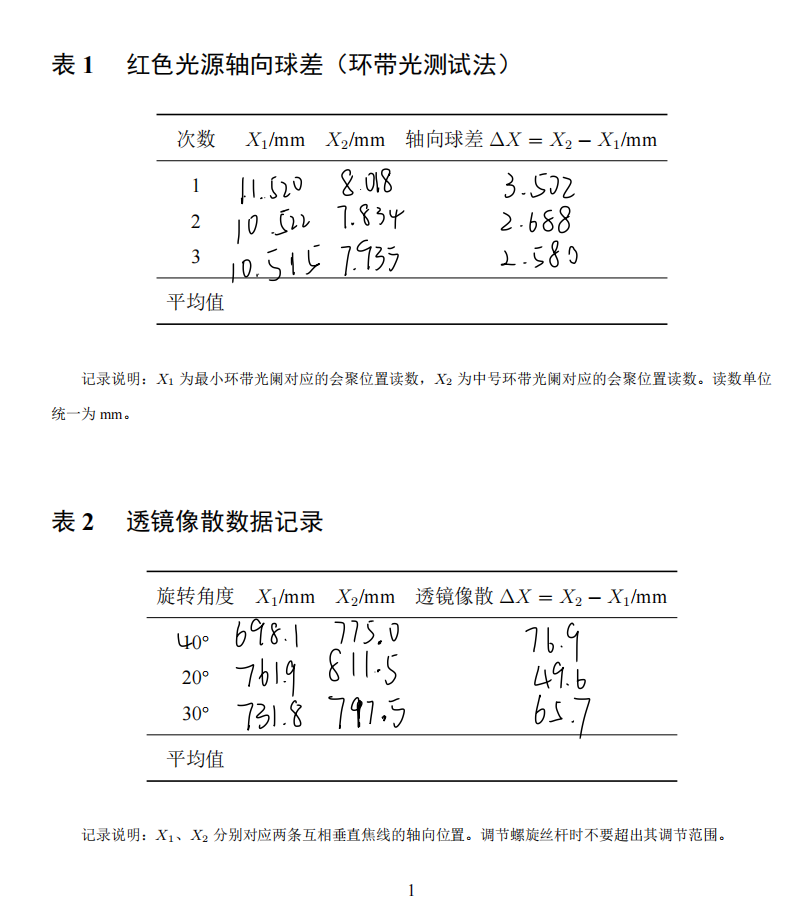
\includegraphics[width=0.85\textwidth]{数据记录单.png}
  \caption{原始数据记录单（学生手写）}
  \label{fig:raw_data}
\end{figure}
\end{document}
